\documentclass{article}
\usepackage[preprint]{neurips_2025}
\makeatletter\renewcommand{\@noticestring}{Tech Report\hfill\href{https://github.com/XizhiXiao/AML-Homework1}{Code: github.com/XizhiXiao/AML-Homework1}}\makeatother
\usepackage[T1]{fontenc}
\usepackage{microtype,amsmath,booktabs,graphicx,xcolor,hyperref,longtable,float}
\hypersetup{colorlinks=true,linkcolor=blue!45!black,urlcolor=blue!45!black}
\title{Pretraining a 0.2B Transformer from Scratch}
\author{Xizhi Xiao\\[4pt]College of AI, Tsinghua University}
\date{Completed experiments: 16 November 2026}
\raggedbottom
\begin{document}
\maketitle
\begin{abstract}
We investigate model scaling and compute allocation by pretraining a 218.97M-parameter Transformer on TinyStories. We implement the model and training pipeline from scratch and use the course reference tokenizer. After 1.049B training tokens, the model achieves a full-validation cross-entropy of 1.1169, perplexity of 3.0554, and 0.4204 bits per byte. Thirty experiments examine scaling at fixed token and compute budgets. At matched training exposure, a power law fitted to five smaller models predicts the main model's loss with 2.08\% relative error. At fixed compute, larger models can perform worse as their available training-token budgets shrink. Across a tenfold increase in compute, selecting the best sampled configuration lowers validation loss by 25.1\%. These results support using small-model experiments to predict larger-model performance and allocating compute jointly to model capacity and training exposure.
\end{abstract}

\section{Part 1: Byte-Level BPE and Training Data}
\subsection{Tokenizer construction}
We implement byte-level BPE to learn a vocabulary directly from text. The tokenizer begins with the 256 UTF-8 byte values. At each iteration, it counts adjacent symbol pairs across training documents and replaces the most frequent pair with a new symbol. Pair frequencies are weighted by document multiplicity, and ties are resolved by symbol IDs. Encoding applies the learned merges in order; decoding concatenates token byte sequences to reconstruct the text. An additional token marks the end of a document (EOS).

The byte alphabet provides coverage of UTF-8 text, while merging frequent sequences allows each token to represent longer recurring fragments. We train the tokenizer on 631 training-side TinyStories documents containing 500,000 bytes. With a target vocabulary of 1,024, training produces $1,024-256-1=767$ merges. The resulting encoding contains 149,926 tokens, or 3.335 bytes per token on the training sample. Thus, the learned merges reduce the sequence length to about 30\% of its byte-level length. Encoding and decoding recover the tested English, multilingual and emoji strings exactly.

\subsection{Corpus preparation}
For language-model training, we use the course reference tokenizer, \texttt{flexitok/bpe\_fw\_edu\_16000}, with a 16,000-token vocabulary. This tokenizer is shared by the main model and all scaling experiments. Our 1,024-token BPE experiment demonstrates vocabulary learning and encoding independently of this training pipeline.

TinyStories documents are separated by an end-of-text line. We assign approximately 99\% to training and 1\% to validation using a deterministic SHA-256 hash of the document text and seed 42. Identical documents receive the same assignment. Each encoded document ends with EOS (ID 2); the token streams are stored as unsigned 16-bit integers and read through memory mapping.



Table~\ref{tab:corpus} summarizes the encoded corpus, which supplies 489.03M training tokens. We use this measured count when interpreting training exposure, and retain original byte counts for bits-per-byte evaluation. Figure~\ref{fig:encoding} records the custom BPE results and a reference-encoding demonstration on 100 documents, which produces 19,282 training tokens and 227 validation tokens.

\begin{table}[H]
\setlength{\abovecaptionskip}{7pt}\setlength{\belowcaptionskip}{7pt}

\centering
\caption{TinyStories statistics under the reference tokenizer. Token counts include EOS.}\label{tab:corpus}
\begin{tabular}{lrrr}\toprule
Split & Documents & Tokens & UTF-8 bytes\\\midrule
Training & 2,098,214 & 489,027,033 & 1,875,600,824\\
Validation & 21,275 & 4,958,034 & 19,004,680\\\bottomrule
\end{tabular}
\end{table}

\begin{figure}[H]\centering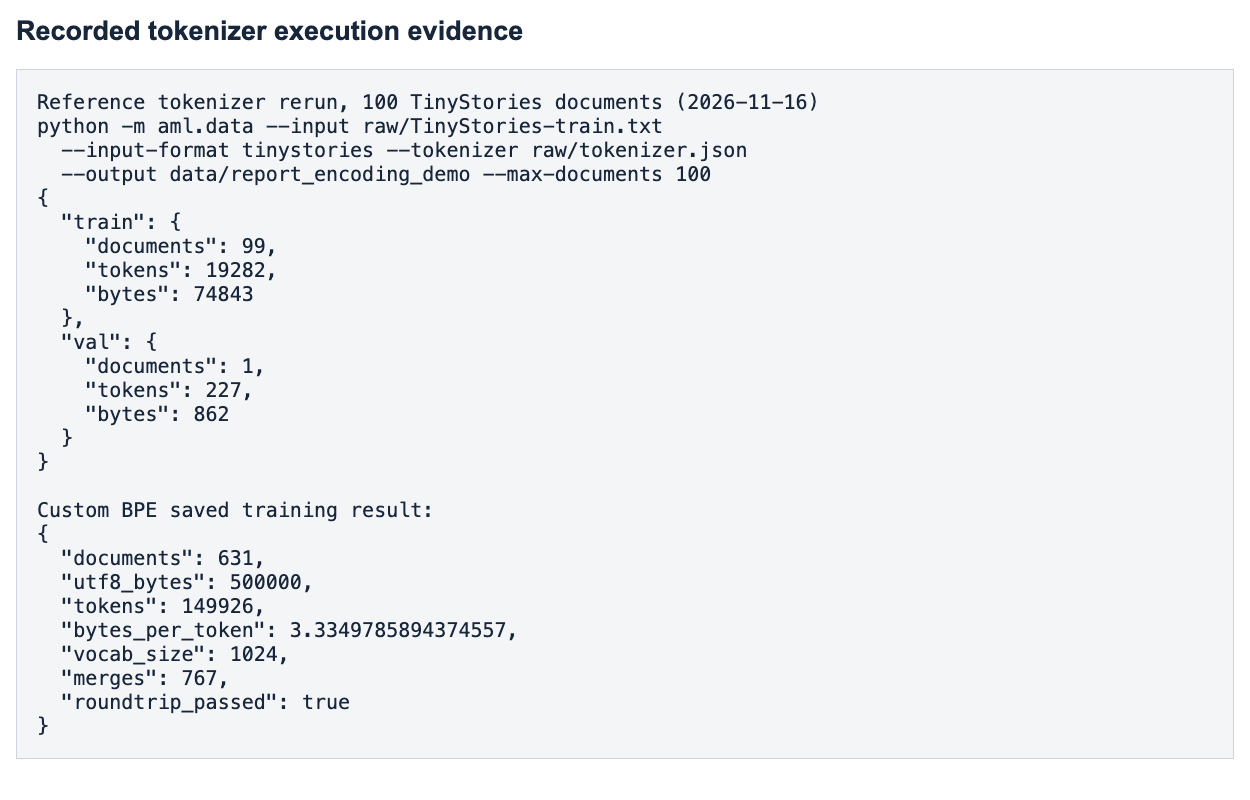
\includegraphics[width=.86\linewidth,trim=0 24 0 0,clip]{figures/tokenization_evidence.png}\caption{Saved BPE results and reference-tokenizer encoding output, displayed in a log viewer.}\label{fig:encoding}\end{figure}

\section{Part 2: Decoder-Only Transformer}
\subsection{Architecture}
We implement the Transformer using PyTorch tensor operations and basic layers, including explicit attention, normalization, residual connections and feed-forward blocks. Token embeddings and learned absolute position embeddings are added before 16 pre-normalized residual blocks. Each block contains causal multi-head self-attention followed by a two-layer GELU feed-forward network:
\begin{align}
H' &= H + \operatorname{Attention}(\operatorname{LN}(H)),\\
H'' &= H' + W_2\operatorname{GELU}(W_1\operatorname{LN}(H')+b_1)+b_2.
\end{align}
Table~\ref{tab:architecture} lists the model dimensions and parameter counts. A final LayerNorm precedes the vocabulary projection. Input embeddings and the output projection share weights. Dropout is set to zero.

\begin{table}[H]
\setlength{\abovecaptionskip}{7pt}\setlength{\belowcaptionskip}{7pt}

\centering
\caption{Main-model configuration and recorded parameter counts.}\label{tab:architecture}
\begin{tabular}{lr@{\hspace{16mm}}lr}\toprule
Setting & Value & Setting & Value\\\midrule
Layers & 16 & Hidden width & 1,024\\
Attention heads & 16 & Head dimension & 64\\
FFN width & 4,096 & Context length & 1,024\\
Vocabulary & 16,000 & Total parameters & 218,974,208\\
 & & Non-embedding parameters & 201,541,632\\\bottomrule
\end{tabular}
\end{table}

\subsection{Causal attention and parameter accounting}
For each head, attention is computed explicitly as
\begin{equation}
\operatorname{Attention}(Q,K,V)=\operatorname{softmax}\!\left(\frac{QK^\top}{\sqrt{64}}+M\right)V,
\qquad M_{ij}=\begin{cases}0 & j\leq i,\\-\infty & j>i.\end{cases}
\end{equation}
The mask prevents a position from accessing future tokens. Softmax is evaluated in FP32 before conversion back to the activation dtype. Head outputs are concatenated and projected to the hidden width. The attention matrix has quadratic space cost in the sequence length.

The non-embedding count excludes both token and position embeddings. Each block contains $12d^2+13d$ parameters for $d_{\mathrm{ff}}=4d$; adding the final LayerNorm gives $16(12d^2+13d)+2d=201{,}541{,}632$. Token and position embeddings add $16{,}000d+1{,}024d$ parameters. The tied output head adds no separate weight matrix.

\subsection{Autoregressive generation}
Generation repeatedly predicts and appends one token. The implementation supports greedy decoding (temperature zero) and temperature-scaled top-$k$ sampling. When the sequence exceeds the context limit, only the most recent 1,024 tokens are retained for prediction, with positions reindexed. Generation recomputes attention over the current context at each step. The examples below use the final best checkpoint, temperature 0.8, top-$k=50$, seed 42, and at most 160 new tokens.

\section{Part 3: Main-Model Training and Evaluation}
\subsection{Training recipe}
The next-token objective is cross-entropy on inputs and targets shifted by one position. Training samples contiguous windows with replacement from the memory-mapped training stream. Windows may cross document boundaries, indicated by EOS. Consequently, processed tokens measure training exposure rather than unique data coverage.



The training recipe in Table~\ref{tab:recipe} uses a budget of 2.14 times the stored token count, with windows sampled independently with replacement. We save the latest checkpoint for resumption and select the best checkpoint by monitoring validation loss. Checkpoints include model weights, optimizer state and random-number states.

\begin{table}[H]
\setlength{\abovecaptionskip}{7pt}\setlength{\belowcaptionskip}{7pt}

\centering
\caption{Completed main-run training recipe.}\label{tab:recipe}
\begin{tabular}{ll}\toprule
Setting & Value\\\midrule
Optimizer & AdamW, $\beta_1=0.9$, $\beta_2=0.95$\\
Weight decay & 0.1 for matrix parameters; zero for biases and normalization\\
Learning rate & Peak $4\times10^{-4}$; 80-step warmup; cosine decay to 10\%\\
Batch & 4 sequences per micro-batch; 64 accumulation steps\\
Tokens per update & $4\times64\times1{,}024=262{,}144$\\
Budget & 4,000 updates; 1,048,576,000 processed tokens\\
Precision / clipping & CUDA BF16 / gradient norm clipped at 1.0\\
Validation / saving & Every 100 updates; best checkpoint by validation loss\\
Monitoring subset & First 128 validation documents\\\bottomrule
\end{tabular}
\end{table}

\clearpage
\subsection{Evaluation protocol}
Each validation document starts from EOS context; every content token and the terminal EOS are predicted. Long documents are divided into context-length chunks, carrying only the preceding token into the next chunk. Padding targets are excluded. This document-wise evaluation scores the same target tokens for every model.

Let $S$ denote the summed negative log-likelihood, $T$ the number of scored target tokens, and $B$ the original UTF-8 byte count over the same documents. We report
\begin{equation}
L=\frac{S}{T},\qquad \mathrm{PPL}=\exp(L),\qquad \mathrm{BPB}=\frac{S}{B\ln 2}.
\end{equation}
Loss is measured in nats per token. EOS contributes to $S$ and $T$, but not to $B$. During training, we evaluate the same first 128 validation documents every 100 updates to track progress and select the best checkpoint at low evaluation cost. After training, we evaluate all 21,275 validation documents to obtain broader coverage of the corpus. Both evaluations use the same scoring method; full-validation results are used for the final model assessment and Part 4 comparisons.


\subsection{Completed results and qualitative assessment}
Figure~\ref{fig:main-metrics} shows the training trajectory, and Table~\ref{tab:main-eval} reports the final evaluation. The run completed all 4,000 steps. Its final training loss was 1.0666; monitoring validation loss declined from 9.8484 at initialization to 1.6843 at step 500, 1.3568 at step 1,000, 1.1900 at step 2,000 and 1.0886 at step 4,000. The final checkpoint was also the best monitoring checkpoint. Validation loss continues to improve through the final update, alongside the decline in training loss.

\begin{table}[H]
\setlength{\abovecaptionskip}{7pt}\setlength{\belowcaptionskip}{7pt}
\centering
\begin{tabular}{lrrr}\toprule Evaluation population & Loss & PPL & BPB\\\midrule
128-document monitoring subset &1.08863&2.97020&0.40833\\
Full validation (21,275 documents)&1.11692&3.05544&0.42039\\\bottomrule\end{tabular}
\caption{Monitoring and final evaluation of the same main-model checkpoint. The subset supports training-time monitoring; the full split provides the final reported result.}\label{tab:main-eval}
\end{table}

\begin{figure}[H]\centering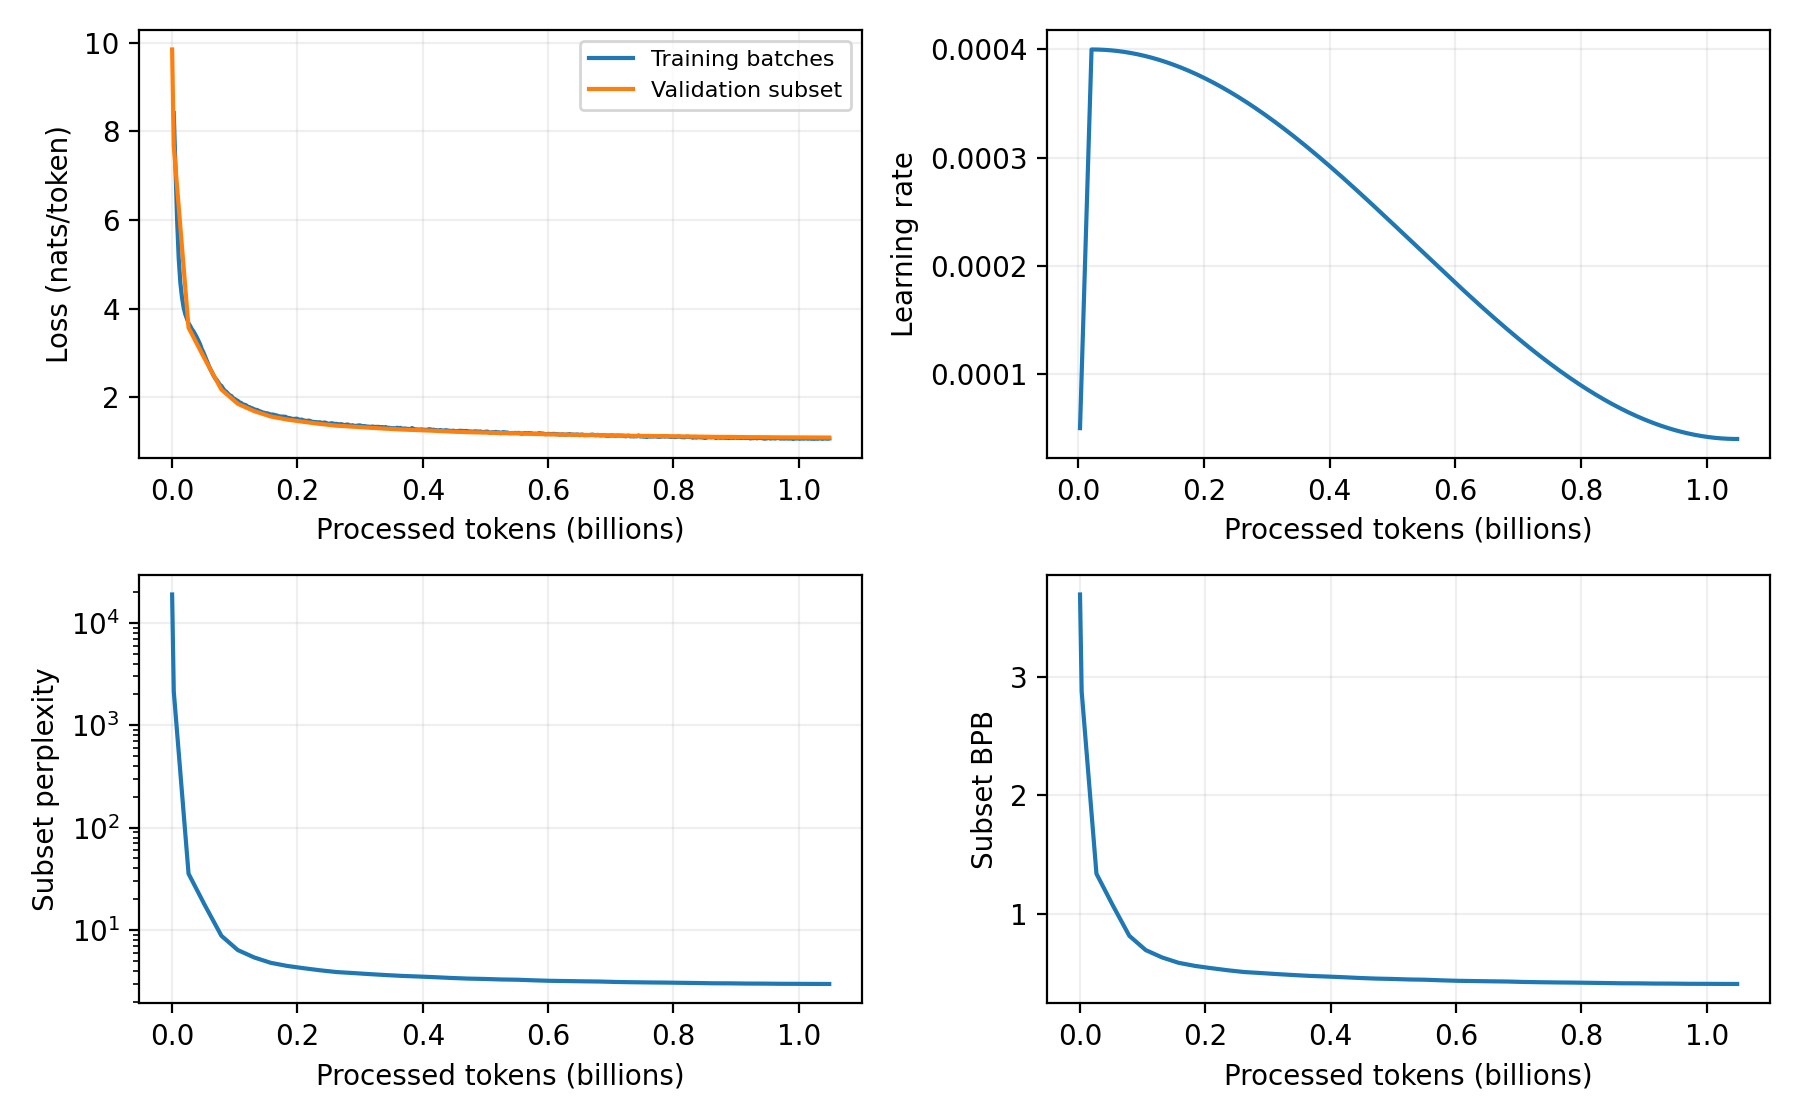
\includegraphics[width=.87\linewidth]{figures/main_metrics.png}\caption{Main-model training metrics and validation metrics on the fixed 128-document monitoring subset.}\label{fig:main-metrics}\end{figure}

\clearpage
The following continuations use temperature 0.8, top-$k=50$ and seed 42, with a limit of 160 new tokens.

\begin{quote}\small
\textbf{Example 1. Prompt:} Once upon a time,

\textbf{Generated continuation:}

there were two friends named Jim and Jill. They loved to ride their bikes together.

One day, the two friends decided to take a break from the bike and go for a walk. Jim and Jill went very slowly and carefully, so they didn't make a single bump in the road.

They soon reached the river and saw some animals swimming in the water. Jim and Jill were very excited and started to ride their bikes through the river.

Suddenly, they spotted a big, green frog. It was very slow and had big eyes.

Jill said to Jim, "Look at that big frog!".

Jim smiled and said, "Let's race the frog, maybe it will join us."

So they hopped on their bikes and
\end{quote}

\begin{quote}\small
\textbf{Example 2. Prompt:} The little girl found

\textbf{Generated continuation:}

that she had to use the soap to wash her hands in the sink. She used a lot of it and the soap became very clean. 

Her mom was very proud. She gave the little girl a big hug and said, "You did a great job washing your hands, my little one! Now you can use the soap to make a special treat for your birthday!" 

The little girl was very excited and with great enthusiasm she went off to make her special surprise. She used the soap to make a big, beautiful flower pot.

When she was done, she proudly presented it to her Mom. Her Mom said, "That's so beautiful! I'm sure it will be a special present for your birthday!" 

The little girl was so happy and was very proud
\end{quote}

Both samples maintain grammatical sentences, dialogue and a simple story structure. In Example 1, the characters switch from walking to riding bicycles through a river. In Example 2, soap becomes a birthday treat and then a flower pot. These transitions illustrate stronger local fluency than commonsense and event consistency. The final sentences reach the generation-length limit. All three outputs and their decoding settings are saved in \texttt{samples.json}.



\begin{figure}[H]\centering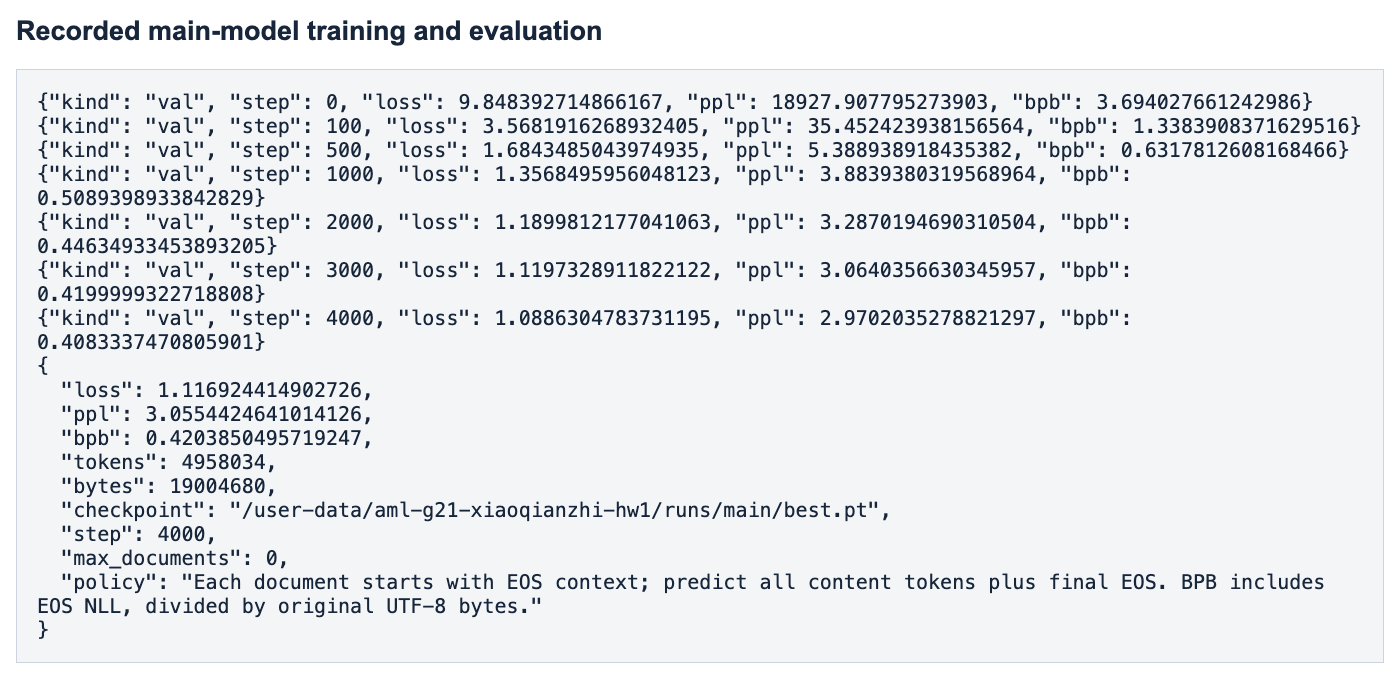
\includegraphics[width=\linewidth,trim=0 20 0 0,clip]{figures/training_evidence.png}\caption{Saved main-model evaluation logs displayed in a log viewer. The upper entries report loss, PPL and BPB on the monitoring subset at selected training steps; the lower entry reports full-validation results for the final checkpoint at step 4,000.}\label{fig:training-log}\end{figure}

\noindent Figure~\ref{fig:training-log} displays selected monitoring records and the final full-validation output. The accompanying files include machine-readable training logs, encoding output, configurations, generated samples and full-validation results. Checkpoint weights are stored separately on the training servers.


\section{Part 4: Scaling Laws, Path 1}
\subsection{Experimental design}
We investigate two questions: how validation loss changes with model size at a fixed training-token budget, and how to allocate a fixed compute budget between model size and training tokens. For the first question, we train five models from 4.74M to 99.23M non-embedding parameters on 1.049B tokens, matching the main model's exposure, and hold out the main model for prediction. Five additional runs at 67.11M tokens measure the effect of a shorter training budget. For the second question, we compare twenty runs across three compute budgets, $10^{16}$, $3\times10^{16}$ and $10^{17}$ FLOPs, with model sizes concentrated around the low-loss regions. Together, these designs comprise thirty runs.

The model configurations in Table~\ref{tab:scaling-models} use the same tokenizer, corpus split, context length of 1,024, tied embeddings and zero dropout. Training uses seed 42, BF16, AdamW, micro-batches of four sequences and eight accumulation steps, giving 32,768 tokens per update. The peak learning rate is $1.4142\times10^{-4}$, with 2\% warmup and cosine decay to 10\% of the peak. Optimizer betas, weight decay and gradient clipping match the main model. The main model uses the larger batch and learning rate in Part 3.

We define $N$ as the non-embedding parameter count and $D$ as processed training tokens, including repeated sampling. Compute is approximated by $C=6ND$, with steps rounded to the nearest update. This convention captures the dominant parameter-dependent training cost; vocabulary projection and attention overhead are excluded. Experiments run on A100 and A40 GPUs using matching corpus and tokenizer hashes.

\begin{table}[H]
\setlength{\abovecaptionskip}{7pt}\setlength{\belowcaptionskip}{7pt}
\centering\small
\begin{tabular}{lrrrr}\toprule Model & Width & Layers & Heads & Exact $N$\\\midrule
1.78M&192&4&3&1,779,840\\2.67M&192&6&3&2,669,568\\5M&256&6&4&4,739,072\\11M&384&6&6&10,647,552\\16.63M&480&6&6&16,627,200\\25M&512&8&8&25,220,096\\50M&512&16&8&50,439,168\\99M&768&14&12&99,231,744\\\bottomrule
\end{tabular}\caption{Model configurations. FFN width is four times hidden width. Refinement scales are used only at selected IsoFLOP budgets.}\label{tab:scaling-models}\end{table}

\subsection{Predicting the main model from smaller models}
Figure~\ref{fig:scaling-fits} (left) shows that, at the 1.049B-token budget, full-validation loss decreases from 1.57243 at 4.74M parameters to 1.14743 at 99.23M. We fit this relation with $L(N)=E+A/N^{\alpha_N}$ using bounded nonlinear least squares and multiple initializations. Each point uses the final checkpoint evaluated on all 21,275 validation documents, with batch size 16 and BF16. The fitted law is
\[L(N)=0.875697+81.749150N^{-0.309949},\quad \mathrm{RMSE}=0.001159.\]
Here $E$ is the fitted asymptote at this training-token budget. The fit predicts a main-model loss of 1.093745, compared with the measured 1.116933: an absolute error of 0.023188 and a relative error of 2.076\%. The model-size range therefore supports a useful prediction of the main model, whose non-embedding parameter count is about twice that of the largest fitting model.

We assess prediction sensitivity in two ways. First, fitting only the four smallest models predicts the held-out 99M model with 0.06\% error. Second, fitting in log-loss space gives a main-model error of 2.05\%, close to the original objective. Table~\ref{tab:prediction} summarizes both hold-out tests.

Leaving one fitting scale out gives main-model predictions between 1.09237 and 1.09647. Across these checks, the prediction remains below the measured loss. The residual gap is consistent across fitting choices; the main model's different batch size and learning rate also affect this comparison.

\begin{table}[H]
\setlength{\abovecaptionskip}{7pt}\setlength{\belowcaptionskip}{7pt}
\centering\small\begin{tabular}{llrrr}\toprule Fit objective & Held-out target & Prediction & Measured & Rel. error\\\midrule
Loss LS & 99M & 1.14679 & 1.14743 & 0.06\%\\
Loss LS & Main & 1.09374 & 1.11693 & 2.08\%\\
Log-loss LS & 99M & 1.14729 & 1.14743 & 0.01\%\\
Log-loss LS & Main & 1.09403 & 1.11693 & 2.05\%\\
\bottomrule\end{tabular}\caption{Prediction results under two fitting objectives. The 99M test fits four smaller models; the main-model test fits all five.}\label{tab:prediction}\end{table}



\begin{figure}[H]\centering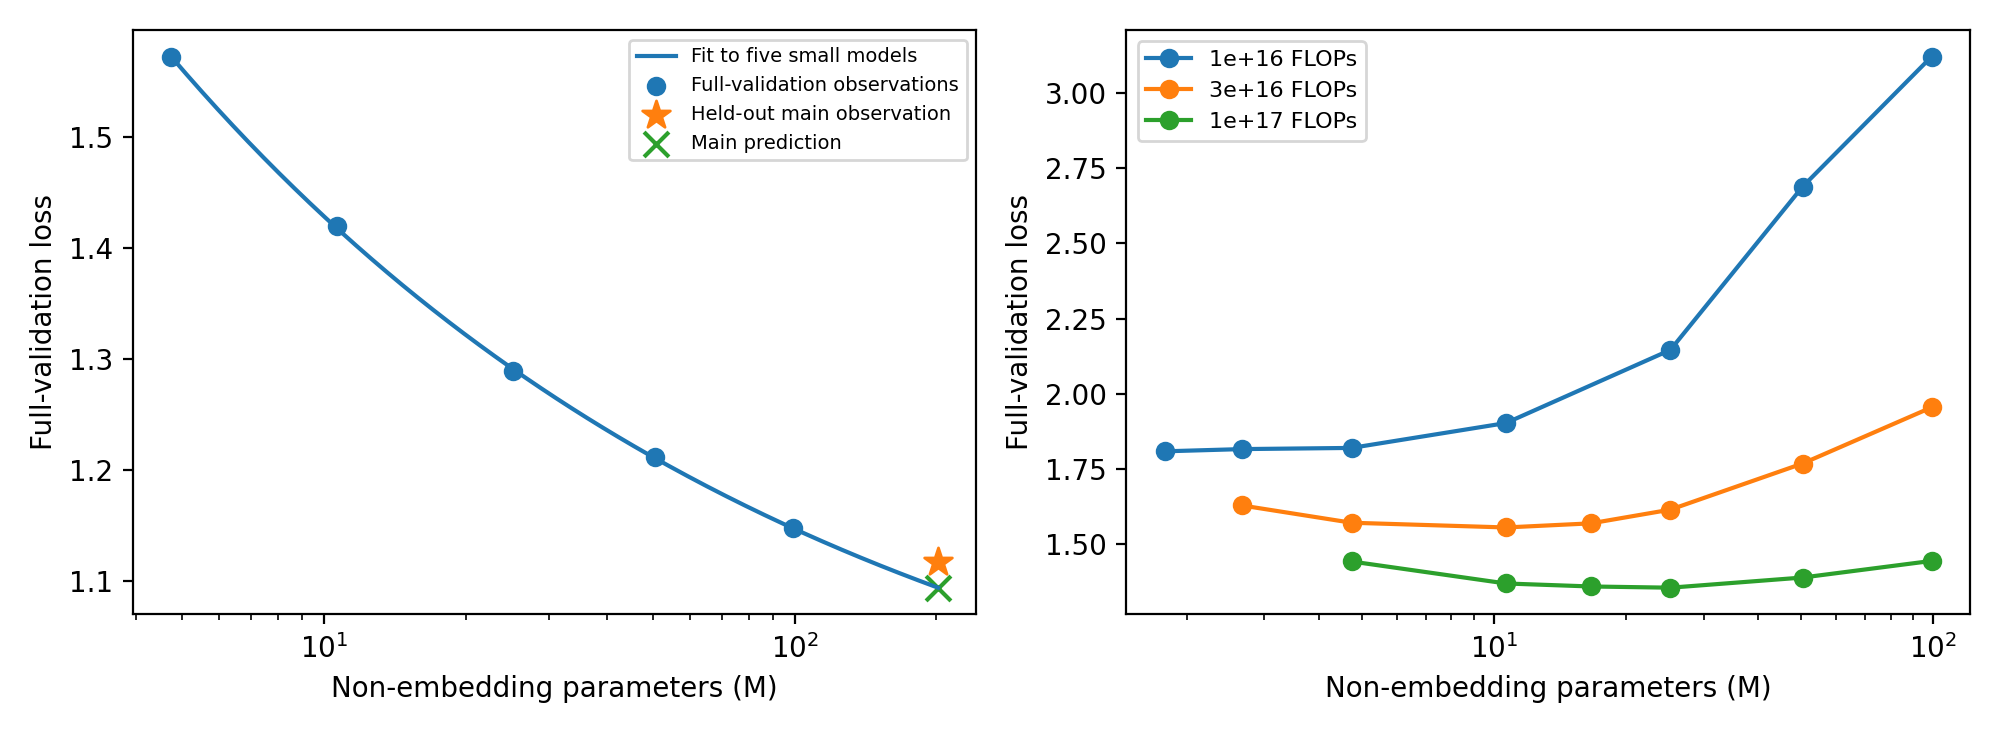
\includegraphics[width=\linewidth]{final_analysis/fits.png}\caption{Full-validation fixed-data extrapolation (left) and IsoFLOP curves including all refinement points (right). The measured main-model point is explicitly shown separately from its prediction.}\label{fig:scaling-fits}\end{figure}

\subsection{Allocating a fixed compute budget}



Table~\ref{tab:isoflop} and Figure~\ref{fig:scaling-fits} (right) show that the lowest-loss sampled model grows with compute: 1.78M parameters at $10^{16}$ FLOPs, 10.65M at $3\times10^{16}$ FLOPs, and 25.22M at $10^{17}$ FLOPs. Their token budgets are 936.41M, 469.60M and 660.87M, respectively. At the middle and highest budgets, loss first falls and then rises as model size increases. Under $C=6ND$, increasing $N$ reduces the available training tokens, producing a trade-off between capacity and training exposure.

The highest-budget curve has a broad low-loss region: 16.63M and 25.22M models achieve losses of 1.35811 and 1.35409, respectively. At the lowest budget, the minimum remains at the smallest sampled model, 1.78M. We therefore report the best sampled configurations, with the lowest-budget optimum constrained by the search boundary and close rankings based on a single seed.

Fitting the three minimum losses yields the compute-performance relation
\[L(C)=190.355923C^{-0.126490},\qquad \mathrm{RMSE}=0.009611.\]
As shown in Figure~\ref{fig:frontier}, over the measured tenfold increase in compute, the best loss falls from 1.80801 to 1.35409, a reduction of 25.1\%. The curve summarizes the improvement achieved by adjusting model size to the available budget.

\begin{table}[H]
\setlength{\abovecaptionskip}{7pt}\setlength{\belowcaptionskip}{7pt}
\centering\small\begin{tabular}{lrrr}\toprule $N$ & $10^{16}$ & $3\times10^{16}$ & $10^{17}$ FLOPs\\\midrule
1.780M & 1.80801 & -- & --\\
2.670M & 1.81544 & 1.62771 & --\\
4.739M & 1.81933 & 1.57031 & 1.44129\\
10.648M & 1.90215 & 1.55457 & 1.36811\\
16.627M & -- & 1.56826 & 1.35811\\
25.220M & 2.14563 & 1.61388 & 1.35409\\
50.439M & 2.68898 & 1.76744 & 1.38790\\
99.232M & 3.12210 & 1.95444 & 1.44321\\
\bottomrule\end{tabular}\caption{Full-validation final losses. Missing combinations were not trained.}\label{tab:isoflop}\end{table}

\begin{figure}[H]\centering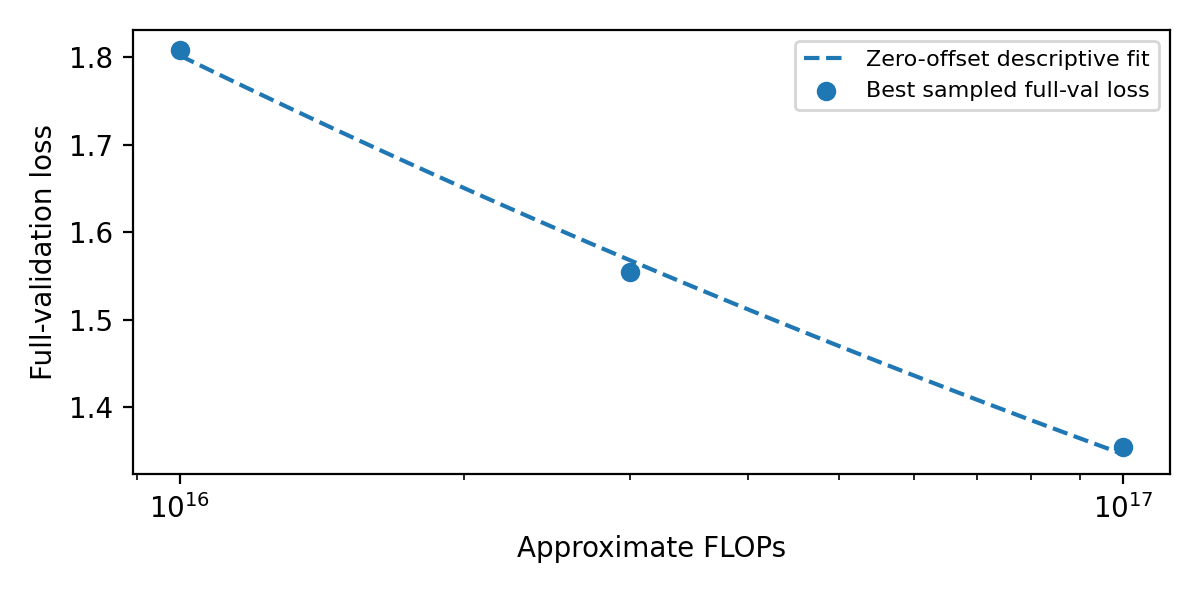
\includegraphics[width=.72\linewidth]{final_analysis/frontier.png}\caption{Best sampled validation loss at each compute budget and a power-law fit to the three points.}\label{fig:frontier}\end{figure}

\subsection{Comparison with Kaplan and Chinchilla Scaling Laws}
We compare our parameter and compute scaling results with the laws reported by Kaplan et al. and Hoffmann et al. (Chinchilla). Kaplan et al.\ [1] report exponents of approximately 0.076 for model size and 0.050 for compute. Hoffmann et al.\ [2] model both parameter and data scaling as $L(N,D)=E+A/N^{0.34}+B/D^{0.28}$. Our fixed-data exponent, 0.310, is numerically close to their parameter exponent. The offset term matters in this comparison: our exponent describes the decay of $L-E$, whereas Kaplan's zero-offset law describes total loss.

Under the Chinchilla formulation, optimizing $N$ and $D$ with $C=6ND$ yields an exponent of $0.34\times0.28/(0.34+0.28)\approx0.154$ for excess loss $L-E$. Our compute exponent of 0.126 instead fits total loss over three budgets. The different dependent quantities, together with TinyStories' domain and our smaller model scales, explain why these exponents should be interpreted within their respective settings.

The fixed-compute curves illustrate the trade-off between model size and training exposure studied in these scaling laws. A larger model helps only when the token budget supports its training. Our best sampled model grows as more compute becomes available, while the precise allocation remains sensitive to the grid: the lowest-budget minimum lies at its boundary and the highest-budget curve is relatively flat around 16.63M--25.22M. These observations support choosing model size jointly with training exposure.

\subsection{Effect of the Training Token Budget}
Figure~\ref{fig:allhist} in the supplementary material shows all thirty validation histories against processed tokens and approximate compute. Monitoring uses the first 128 validation documents; final model comparisons use the full validation split. Table~\ref{tab:all-runs} lists the final results for all thirty runs. At 67.11M tokens, increasing model size from 4.74M to 99.23M reduces final full-validation loss from 2.88523 to 1.77466. Extending training to 1.049B tokens lowers these losses to 1.57243 and 1.14743. Training exposure improves performance at both ends of the model-size range.

\clearpage
\section{Conclusion}
We built a language-model pretraining pipeline comprising byte-level BPE, a decoder-only Transformer, training, evaluation and autoregressive generation. The custom BPE learns 767 merges to form a 1,024-token vocabulary. Using the course reference tokenizer for model training, the 218.97M-parameter Transformer reaches a full-validation loss of 1.1169, perplexity of 3.0554 and BPB of 0.4204 after 1.049B training tokens (Table~\ref{tab:main-eval}). Its continuations reproduce the grammar and dialogue of short stories, while event consistency remains a visible weakness.

The scaling experiments show how model size and training exposure jointly affect performance. At a fixed token budget, a power law fitted to five smaller models predicts the main-model loss with 2.08\% relative error (Table~\ref{tab:prediction}). At fixed compute, increasing model size eventually reduces performance as the available training tokens decrease. Selecting the best sampled configuration at each budget reduces loss from 1.8080 to 1.3541 across a tenfold increase in compute (Figure~\ref{fig:frontier}). These results support using small-model experiments to estimate larger-model performance and choosing model capacity together with the training-token budget.

\normalsize\section*{References}
\begin{enumerate}\small
\item Kaplan et al. (2020). Scaling Laws for Neural Language Models. \url{https://arxiv.org/abs/2001.08361}.
\item Hoffmann et al. (2022). Training Compute-Optimal Large Language Models. \url{https://arxiv.org/abs/2203.15556}.
\item Eldan and Li (2023). TinyStories. \url{https://arxiv.org/abs/2305.07759}.
\item Sennrich et al. (2016). Neural Machine Translation of Rare Words with Subword Units. \url{https://arxiv.org/abs/1508.07909}.
\item Vaswani et al. (2017). Attention Is All You Need. \url{https://arxiv.org/abs/1706.03762}.
\item Assignment 1; lectures A2.2 (Transformer), A3 (Scaling); course reference tokenizer \url{https://huggingface.co/flexitok/bpe_fw_edu_16000}.
\end{enumerate}

\section*{AI Assistance}
AI tools assisted with implementation, debugging, experiment execution, and report editing. The author directed the study, made decisions on experimental scope, and reviewed and revised the analysis and presentation.


\clearpage

\section*{Supplementary Material}
\subsection*{S1. Training Trajectories}
\begin{figure}[H]\centering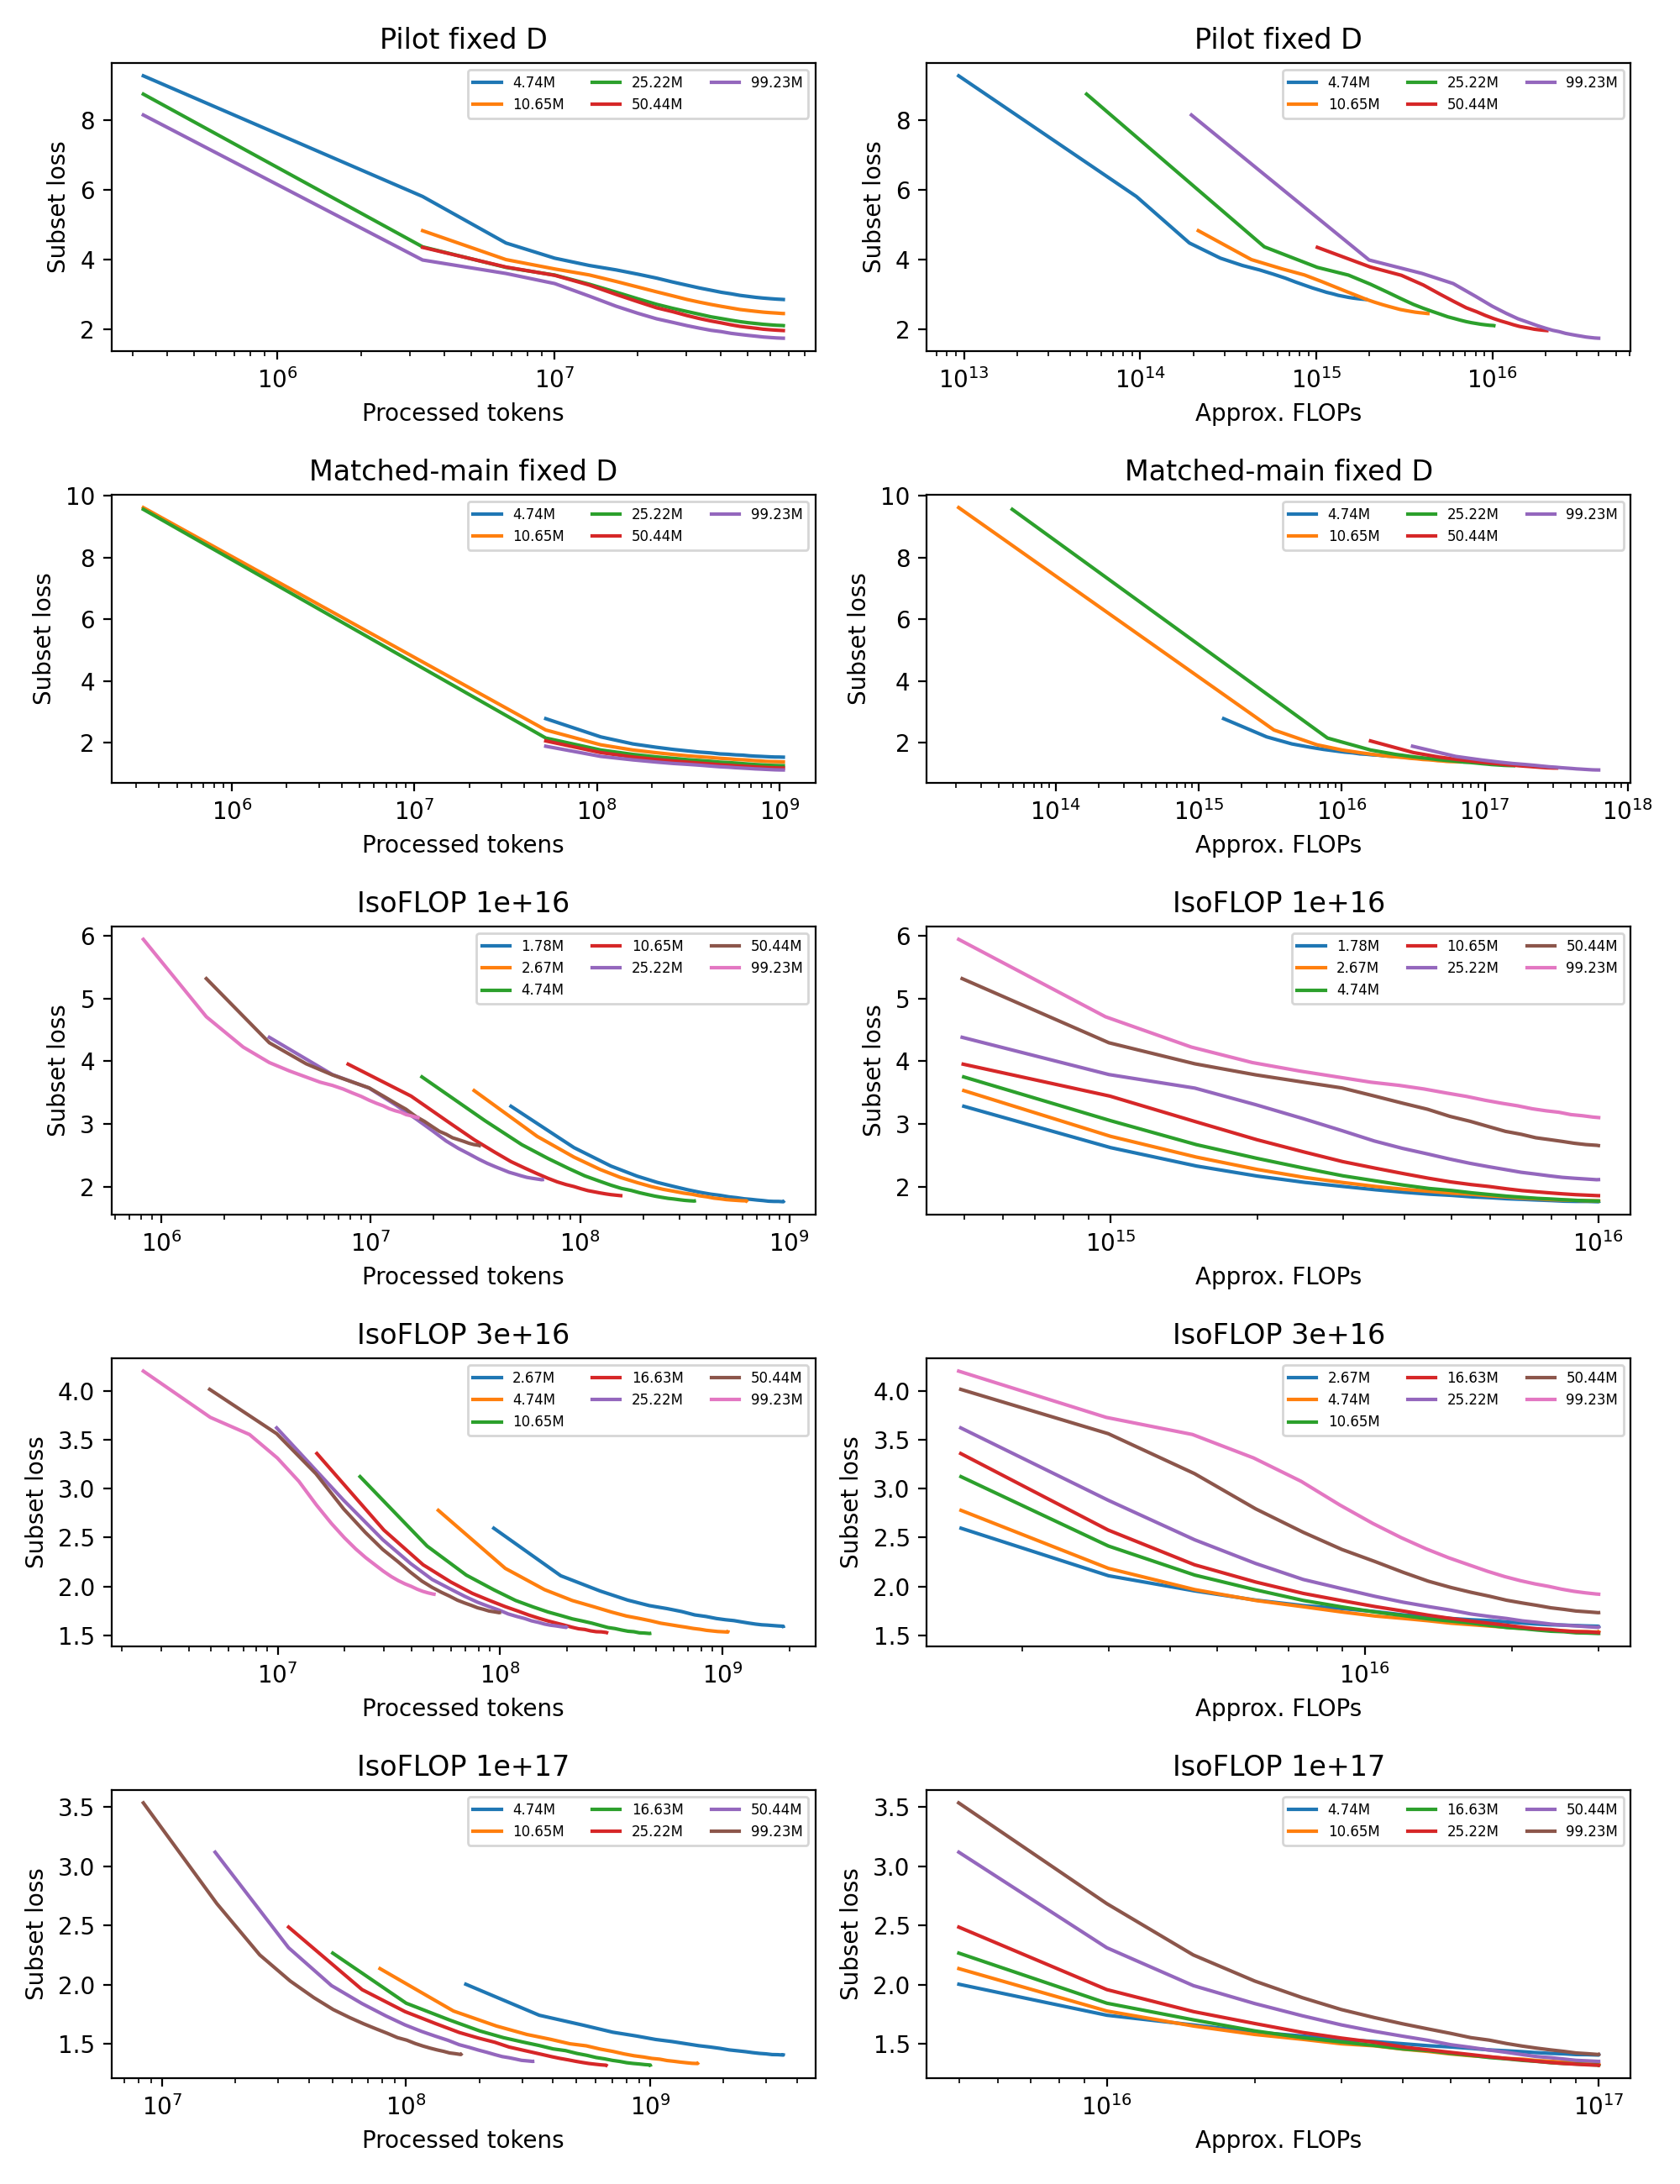
\includegraphics[width=.95\linewidth,height=.80\textheight,keepaspectratio]{final_analysis/all_30_histories.png}\caption{All 30 monitoring validation trajectories, grouped by experimental design. Horizontal axes are log-scaled.}\label{fig:allhist}\end{figure}

\clearpage
\subsection*{S2. Detailed Experimental Results}
\normalsize\renewcommand{\arraystretch}{1.45}
\begin{longtable}{lrrrrr}
\caption{Training budgets and final validation losses for all thirty scaling runs.}\label{tab:all-runs}\\[7pt]
\toprule Cohort & $N$ (M) & $D$ (M) & $C/10^{16}$ & Subset $L$ & Full $L$\\\midrule
Main fixed $D$ & 4.739 & 1048.576 & 2.9816 & 1.53605 & 1.57243\\
Main fixed $D$ & 10.648 & 1048.576 & 6.6989 & 1.38293 & 1.41978\\
Main fixed $D$ & 25.220 & 1048.576 & 15.8671 & 1.26069 & 1.28907\\
Main fixed $D$ & 50.439 & 1048.576 & 31.7336 & 1.18386 & 1.21131\\
Main fixed $D$ & 99.232 & 1048.576 & 62.4312 & 1.12173 & 1.14743\\
IsoFLOP & 1.780 & 936.411 & 1.0000 & 1.76962 & 1.80801\\
IsoFLOP & 2.670 & 624.329 & 1.0000 & 1.78198 & 1.81544\\
IsoFLOP & 4.739 & 351.699 & 1.0000 & 1.78013 & 1.81933\\
IsoFLOP & 10.648 & 156.533 & 1.0000 & 1.86520 & 1.90215\\
IsoFLOP & 25.220 & 66.093 & 1.0001 & 2.11999 & 2.14563\\
IsoFLOP & 50.439 & 33.030 & 0.9996 & 2.66124 & 2.68898\\
IsoFLOP & 99.232 & 16.810 & 1.0009 & 3.10560 & 3.12210\\
IsoFLOP & 2.670 & 1872.953 & 3.0000 & 1.59078 & 1.62771\\
IsoFLOP & 4.739 & 1055.064 & 3.0000 & 1.53490 & 1.57031\\
IsoFLOP & 10.648 & 469.598 & 3.0000 & 1.51817 & 1.55457\\
IsoFLOP & 16.627 & 300.712 & 3.0000 & 1.52740 & 1.56826\\
IsoFLOP & 25.220 & 198.246 & 2.9999 & 1.58247 & 1.61388\\
IsoFLOP & 50.439 & 99.123 & 2.9998 & 1.73128 & 1.76744\\
IsoFLOP & 99.232 & 50.397 & 3.0006 & 1.92004 & 1.95444\\
IsoFLOP & 4.739 & 3516.858 & 10.0000 & 1.40607 & 1.44129\\
IsoFLOP & 10.648 & 1565.295 & 9.9999 & 1.33401 & 1.36811\\
IsoFLOP & 16.627 & 1002.373 & 10.0000 & 1.32058 & 1.35811\\
IsoFLOP & 25.220 & 660.865 & 10.0002 & 1.31933 & 1.35409\\
IsoFLOP & 50.439 & 330.433 & 10.0000 & 1.35187 & 1.38790\\
IsoFLOP & 99.232 & 167.969 & 10.0007 & 1.41095 & 1.44321\\
Short fixed $D$ & 4.739 & 67.109 & 0.1908 & 2.85386 & 2.88523\\
Short fixed $D$ & 10.648 & 67.109 & 0.4287 & 2.45025 & 2.47957\\
Short fixed $D$ & 25.220 & 67.109 & 1.0155 & 2.10290 & 2.12956\\
Short fixed $D$ & 50.439 & 67.109 & 2.0309 & 1.96067 & 1.99674\\
Short fixed $D$ & 99.232 & 67.109 & 3.9956 & 1.74084 & 1.77466\\
\bottomrule\end{longtable}
\end{document}